\documentclass[11pt,aspectratio=169]{beamer}
\usepackage[utf8]{inputenc}
\usepackage[T1]{fontenc}
\usetheme{default}
\usepackage{pdfpcnotes}
\usepackage{todonotes}
\usepackage{xspace}
%checkmarks
\usepackage{pifont}
\usepackage{bbding}
\newcommand{\xmark}{\ding{55}}%
% toprule, midrule, bottomrule
\usepackage{booktabs}
\usepackage{caption}

\usepackage{tikz}
\usetikzlibrary{arrows,shapes,calc}

% 'frame' option for figures
\usepackage[export]{adjustbox}

\usepackage{adjustbox}

% MAMID macro
\newcommand{\mamid}{\textit{MAMID}\xspace}

%done checkmark
\definecolor{darkgreen}{rgb}{0.0, 0.5, 0.0}
\newcommand{\checkcomment}[1]{%
    \def\temp{#1}%
    \ifx\temp\empty%
    \emph{}%
    \else%
    \emph{Note: #1}%
    \fi%
}%
\newcommand{\done}[1][]{{\color{darkgreen}\checkmark\checkcomment{#1}}}
\newcommand{\notdone}[1][]{{\color{red}\xmark\checkcomment{#1}}}

% http://tex.stackexchange.com/questions/279100/typeset-the-shrug-%C2%AF-%E3%83%84-%C2%AF-emoji

\newcommand{\shrug}[1][]{%
\begin{tikzpicture}[baseline,x=0.8\ht\strutbox,y=0.8\ht\strutbox,line width=0.125ex,#1]
\def\arm{(-2.5,0.95) to (-2,0.95) (-1.9,1) to (-1.5,0) (-1.35,0) to (-0.8,0)};
\draw \arm;
\draw[xscale=-1] \arm;
\def\headpart{(0.6,0) arc[start angle=-40, end angle=40,x radius=0.6,y radius=0.8]};
\draw \headpart;
\draw[xscale=-1] \headpart;
\def\eye{(-0.075,0.15) .. controls (0.02,0) .. (0.075,-0.15)};
\draw[shift={(-0.3,0.8)}] \eye;
\draw[shift={(0,0.85)}] \eye;
% draw mouth
\draw (-0.1,0.2) to [out=15,in=-100] (0.4,0.95); 
\end{tikzpicture}}


% insert section title at \section{}
% http://tex.stackexchange.com/questions/178800/creating-sections-each-with-title-pages-in-beamers-slides
\AtBeginSection[]{
    \begin{frame}
        \vfill
        \centering
        \begin{beamercolorbox}[sep=8pt,center,shadow=true,rounded=true]{title}
            \usebeamerfont{title}\insertsectionhead\par%
        \end{beamercolorbox}
        \vfill
    \end{frame}
}

% For tikz highlighting
\tikzset{onslide/.code args={<#1>#2}{%
    \only<#1>{\pgfkeysalso{#2}} % \pgfkeysalso doesn't change the path
}}

\newcommand{\mamidscreenshot}[1]{\includegraphics[width=\textwidth,frame]{#1}}

\newcommand{\clusterlayoutbase}
{
    \tikzstyle{host} = [draw, thin, minimum width=160pt, minimum height=40pt]
    \tikzstyle{slave} = [draw, thin, minimum width=160pt, minimum height=40pt]
    \tikzstyle{mongod} = [draw, thin, minimum width=80pt, minimum height=40pt]
    \tikzstyle{psu} = [draw, ellipse, thin, minimum width=60pt, minimum height=40pt]
    \tikzstyle{repl} = [draw, ellipse, thin, minimum width=60pt, minimum height=40pt]
    \tikzstyle{alert} = [draw, fill=red!50, fill opacity=0.5]
    \path[->] coordinate (host0) {};
    \foreach \h in {1,...,6}
    {
        \path[->] node[host, anchor=east] at ($(host0.east) + (190pt * \h, 0)$) (host\h) {Host \h};
        \path[->] node[slave, anchor=south] at ($(host\h.north)$) (slave\h) {Slave};
        \foreach \m in {1,...,2}
        {
            \path[->] node[mongod, anchor=south east] at ($(slave\h.north west) + (80pt * \m, 0)$) (mongod\h-\m) {mongod};
        }
    }
    \path[->] coordinate (hostn) at ($(host6.east)$) {};
    \foreach \p in {1,...,3}
    {
        \pgfmathtruncatemacro{\refh}{\p * 2 - 1}
        \pgfmathtruncatemacro{\lasth}{\refh + 1}
        \path[->] node[psu, anchor=north] (psu\p) at ($(host\refh.south)!0.5!(host\lasth.south) + (0, -30pt)$) {PSU \p};
        \foreach \hc in {0,...,1}
        {
            \pgfmathtruncatemacro{\host}{\refh + \hc}
            \path[-] (host\host) edge (psu\p);
        }
    }
 
    \foreach \r in {1,...,4}
    {
        \pgfmathsetmacro{\pos}{(\r-0.5)/4}
        \path[->] node[repl, anchor=south] (repl\r) at ($(host0)!\pos!(hostn) + (0, 160pt)$) {Replica Set \r};
    }
}
\newcommand{\clusterlayoutdumbreplicasets}
{
    \path[-] (mongod1-1.north) edge (repl1);
    \path[-] (mongod1-2.north) edge (repl1);
    \path[-] (mongod2-1.north) edge (repl1);

    \path[-] (mongod2-2.north) edge (repl2);
    \path[-] (mongod3-1.north) edge (repl2);
    \path[-] (mongod3-2.north) edge (repl2);

    \path[-] (mongod4-1.north) edge (repl3);
    \path[-] (mongod4-2.north) edge (repl3);
    \path[-] (mongod5-1.north) edge (repl3);

    \path[-] (mongod5-2.north) edge (repl4);
    \path[-] (mongod6-1.north) edge (repl4);
    \path[-] (mongod6-2.north) edge (repl4);
}
\newcommand{\clusterlayoutsmartreplicasets}
{
    \path[-] (mongod1-1.north) edge (repl1);
    \path[-] (mongod3-1.north) edge (repl1);
    \path[-] (mongod5-1.north) edge (repl1);

    \path[-] (mongod1-2.north) edge (repl2);
    \path[-] (mongod3-2.north) edge (repl2);
    \path[-] (mongod5-2.north) edge (repl2);

    \path[-] (mongod2-1.north) edge (repl3);
    \path[-] (mongod4-1.north) edge (repl3);
    \path[-] (mongod6-1.north) edge (repl3);

    \path[-] (mongod2-2.north) edge (repl4);
    \path[-] (mongod4-2.north) edge (repl4);
    \path[-] (mongod6-2.north) edge (repl4);
}


\begin{document}
   	\author{Niklas Fuhrberg, Anton Schirg,\\ Christian Schwarz, Janis Streib, Bob Weinand}
    \title{MAMID}
    \subtitle{Monitor and Manager for In-memory Databases}
    %\logo{}
    \institute{\textbf{Supervisor}\\Dr Marek Szuba\\SCC}
    \date{12 September 2016}
    \subject{Final Presentation}
    %\setbeamercovered{transparent}
    %\setbeamertemplate{navigation symbols}{}
    
    \frame[plain]{\maketitle}

    \begin{frame}<1>[label=waterfall]{PSE: Where are we?}
        \tikzstyle{phase} = [draw, thin,text width={width("Requirements Elicitation")}]
        \tikzstyle{artifact} = [draw, rounded corners=0.1cm, thin,font=\tiny]
        \tikzstyle{alert} = [fill=red!20]
        \begin{figure}
            \begin{tikzpicture}[node distance=1cm, auto,>=latex', thick, align=center]
                \path[->] node[phase, onslide=<1>{alert}] (elicitation) {Requirements Elicitation};
                \path[->] node[phase, onslide=<2>{alert}, right of=elicitation, below of=elicitation] (analysis) {Requirements Analysis}
                          (elicitation) edge (analysis);
                \path[->] node[phase, onslide=<3>{alert}, right of=analysis, below of=analysis] (design) {Design}
                          (analysis) edge (design);
                \path[->] node[phase, onslide=<4>{alert}, right of=design, below of=design] (implementation) {Implementation}
                          (design) edge (implementation);
                \path[->] node[phase, onslide=<4>{alert}, right of=implementation, below of=implementation] (testing) {Testing}
                          (implementation) edge (testing);
                \path[->] node[phase, onslide=<5>{alert}, right of=testing, below of=testing] (acceptance) {Acceptance}
                          (testing) edge (acceptance);
                    \draw[->] (analysis) [out=0,in=100,looseness=0.75] to node[artifact]{Functional\\Specification} ($(design.north east) - (0.25cm, 0)$);
                    \draw[->] (design) [out=0,in=100,looseness=0.75] to node[artifact]{Class Diagram\\Design Document} ($(implementation.north east) - (0.25cm, 0)$);
                    \draw[->] (implementation) [out=0,in=100,looseness=0.75] to node[artifact]{Implementation \&\\Testing Report} ($(acceptance.north east) - (0.25cm, 0)$);
            \end{tikzpicture}
        \end{figure}
    \end{frame}
    
    \section{Requirements Elicitation}
    
    \begin{frame}{Motivation}
        \begin{itemize}
            \item Envisat earth observation satellite
            \item Archive of data from MIPAS instrument\pnote{MIPAS records trace gasses in the atmosphere}
            \item Research project at IMK: %TODO what is its name?
            \item \pnote{Original data not that big but }Processed data: $96+$ TB
            \item Periodic reprocessing \& archiving \pnote{Reprocessing happens periodically, old results need to be kept for reference purposes => dataset is growing}
            \item Use MongoDB for storage\pnote{use MongoDB's sharding feature (more in a second) to distribute the data over multiple machines, easy way to access data and use it in downstream applications}
        \end{itemize}
    \end{frame}
    
    \begin{frame}{MongoDB}
        TODO
        \begin{itemize}
            \item MongoDs / Mongods
            \item Replica Set
            \item Sharding
        \end{itemize}
    \end{frame}
    
    \begin{frame}[allowframebreaks]{MongoDB on IMK Cluster}
        
        \begin{figure}
        \end{figure}
            \begin{adjustbox}{max totalsize={.9\textwidth}{.7\textheight},center}
                \huge
            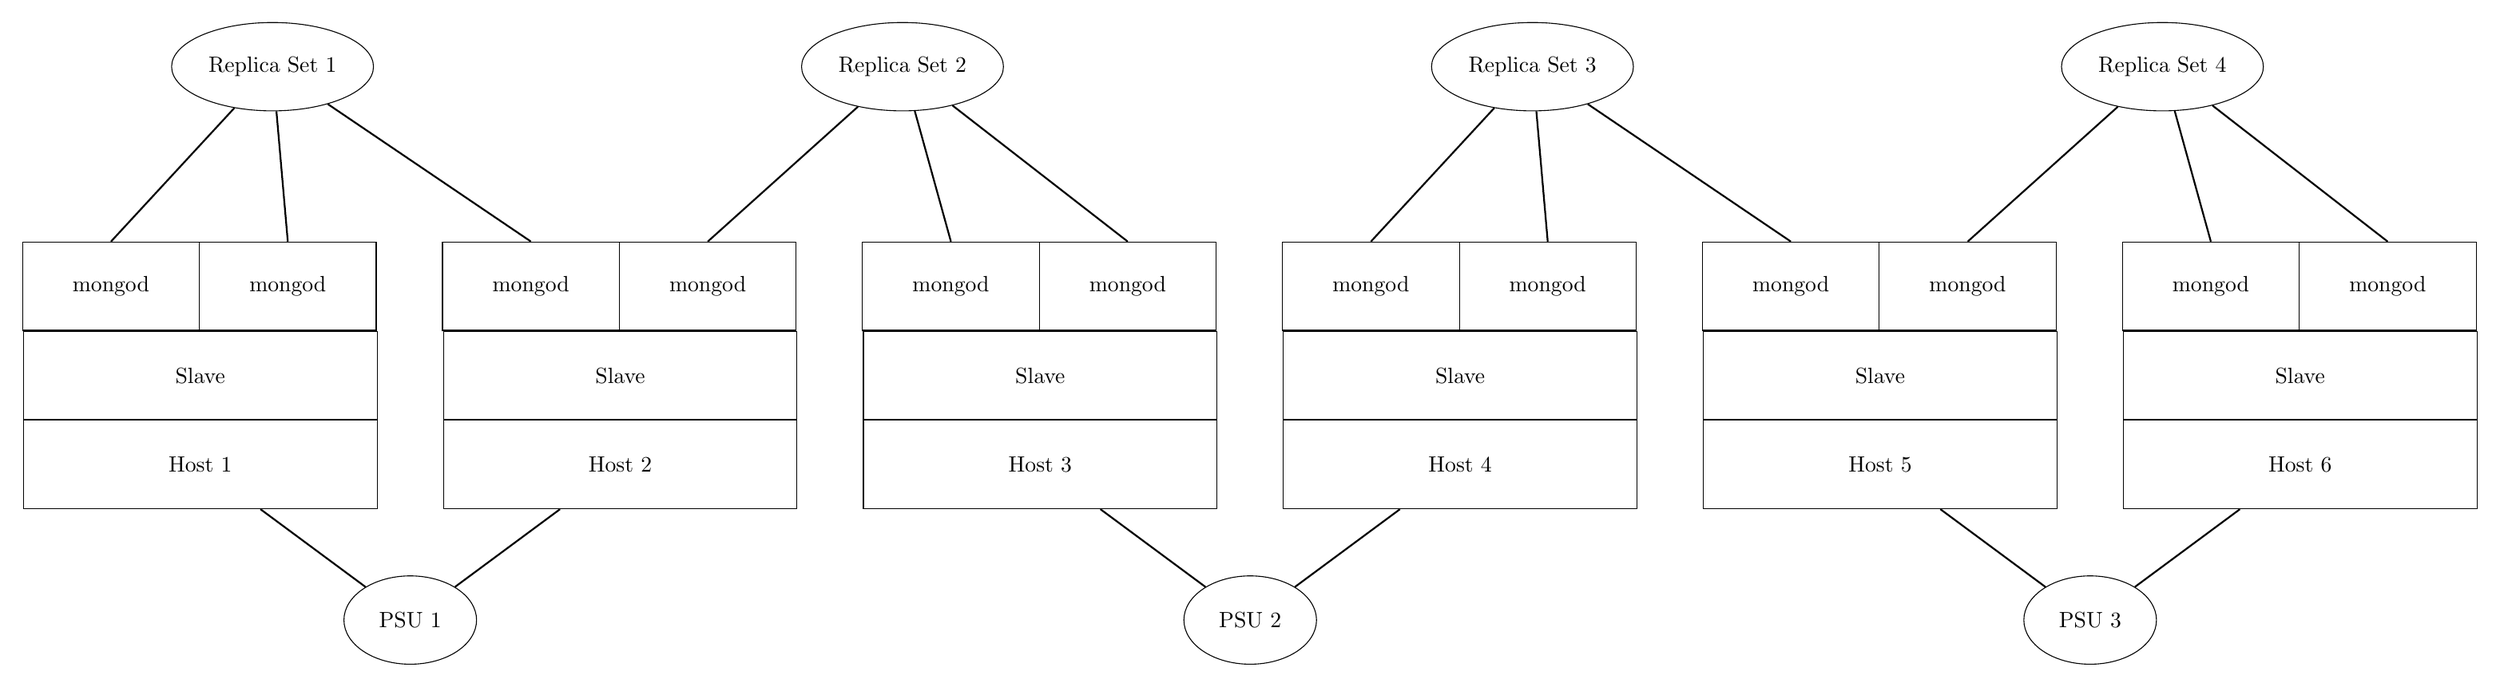
\begin{tikzpicture}[node distance=1cm, auto,>=latex', thick]
                \clusterlayoutbase
                \clusterlayoutdumbreplicasets
            \end{tikzpicture}
            \end{adjustbox}
        \begin{itemize}
            \item Few big machines with (slow?) persistent storage\\%TODO ask marek whcih one it is
                  + 4 cabinets à 20 blades à $98$ GB RAM %TODO check this
            \item Runs OpenIndiana \pnote{openindiana, who has heard of it? it's an illumos distro. which is? anyone??}
            \item Blades have small boot-only HDDs
            \item Cabinets have independent PSUs
        \end{itemize}

        \framebreak
        
        Performance: Replica Sets \pnote{so what can we do to maximize performance, in particular read performance for downstream applications?}
        
        \begin{itemize}
            \item Primaries: on blades with in-memory storage (\emph{performance})
            \item Secondaries: on machines with HDDs (\emph{persistence}) \pnote{this can be arranged by configuring the Priority of a Mongod in Replica Set elections}
        \end{itemize}
        \pnote{indicate where primaries and secondaries go using a pointing device}
        \begin{figure}
            \begin{adjustbox}{max totalsize={.9\textwidth}{.7\textheight},center}
                \huge
            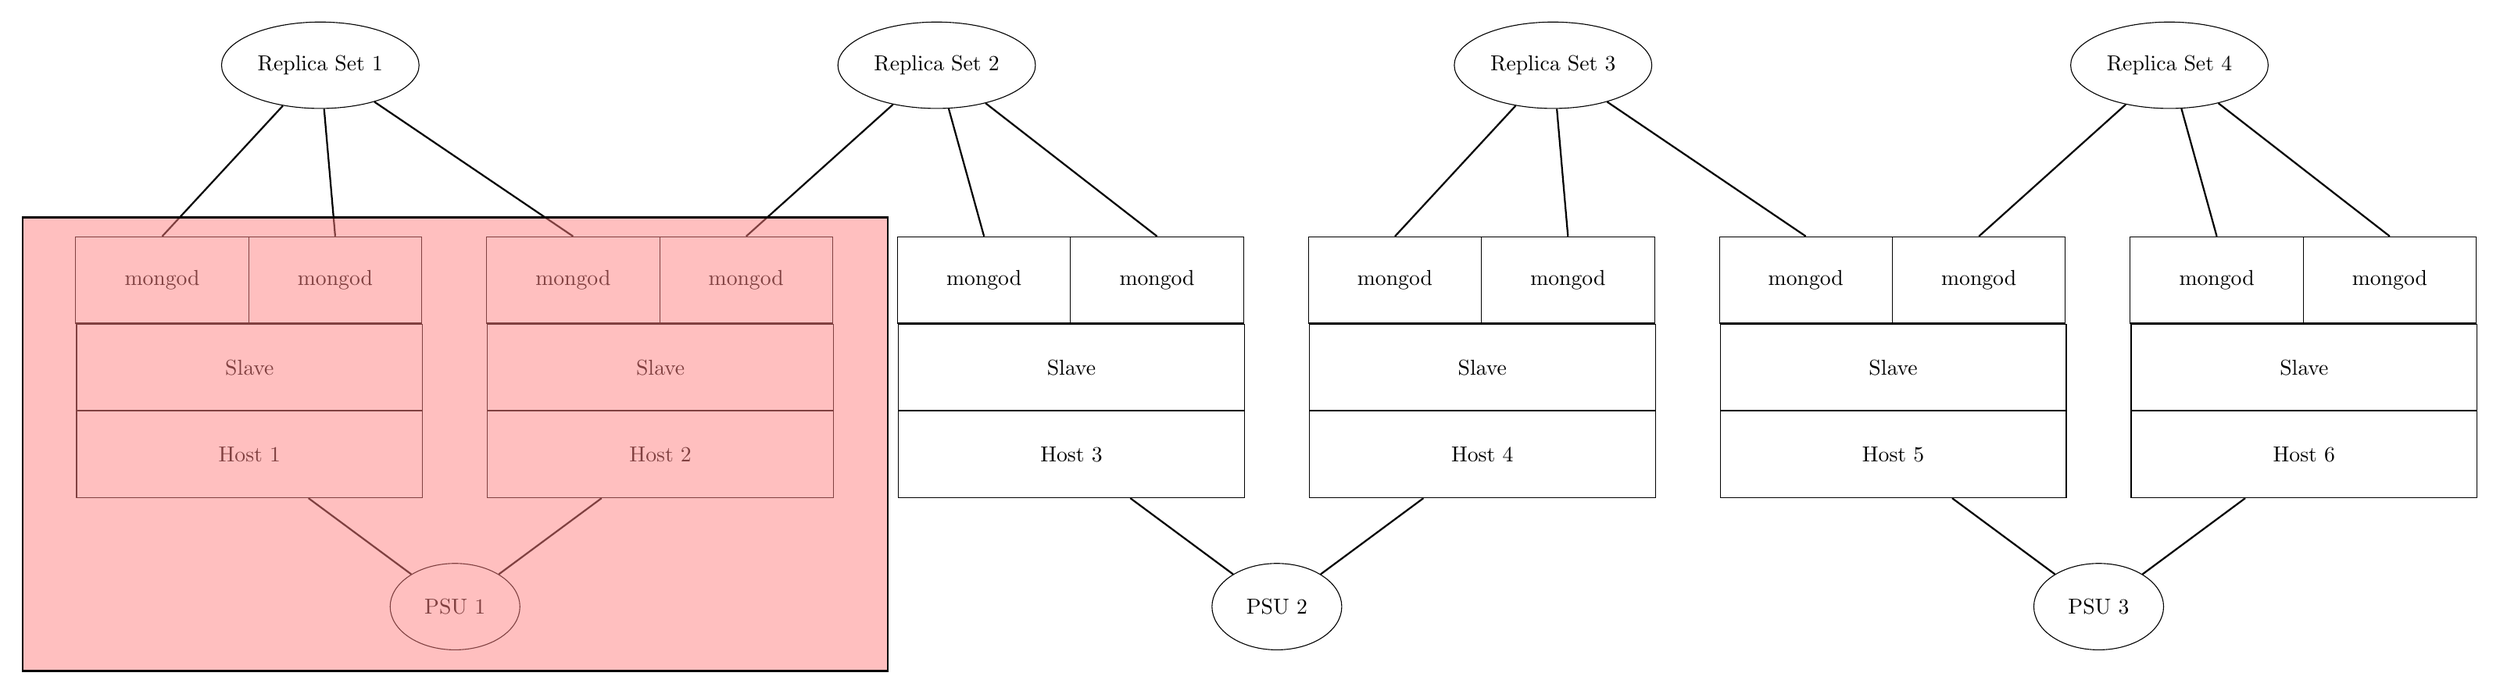
\begin{tikzpicture}[node distance=1cm, auto,>=latex', thick]
                \clusterlayoutbase
                \clusterlayoutdumbreplicasets
                \path[->] node[alert, anchor=south, minimum height=210pt, minimum width=400pt] (psudown) at ($(psu1.south) + (0, -10pt)$) {};
            \end{tikzpicture}
            \end{adjustbox}
        \end{figure}
        
        \framebreak
        
        Availability \& Redundancy: Risk Groups \pnote{so far we have performance, but what happens in case a PSU dies and takes a cabinet offline?}
        
        \begin{itemize}
            \item Distribute Replica Set members over different cabinets
            \item Assert enough Replica Set members have persistent storage\pnote{requirements may vary, depending on importance of data, ... generally a tradeoff between space usage and safety}
        \end{itemize}
        
        \begin{figure}
            \begin{adjustbox}{max totalsize={.9\textwidth}{.7\textheight},center}
                \huge
            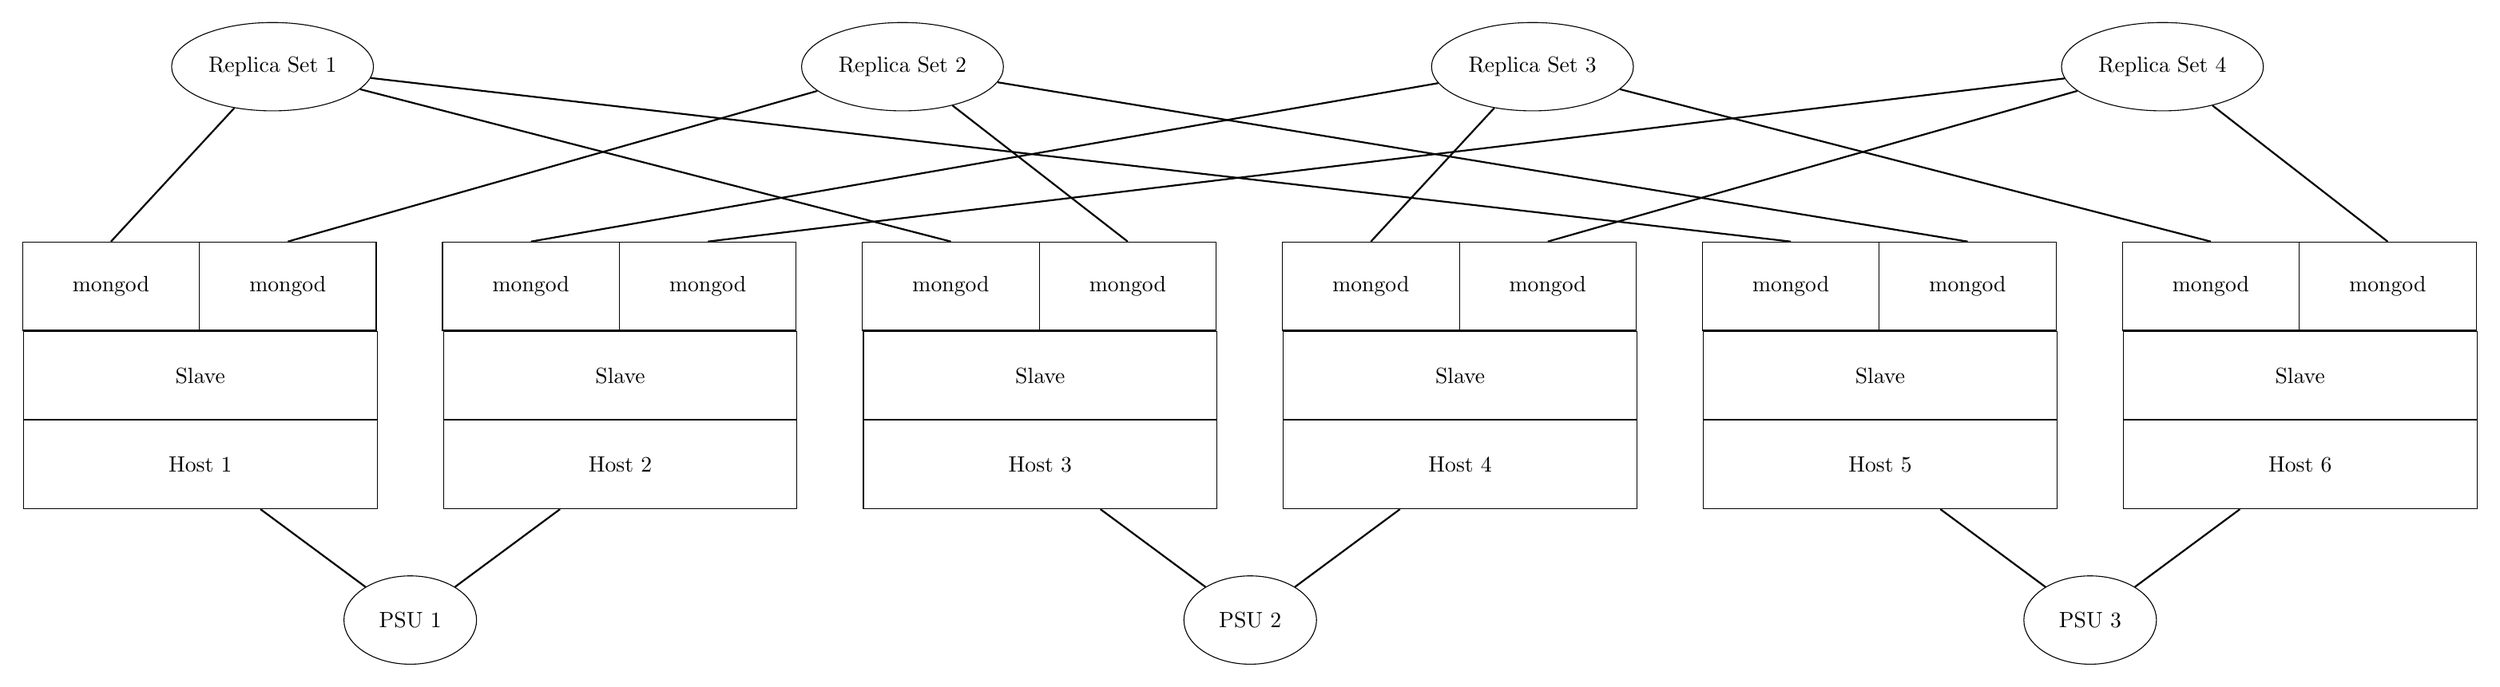
\begin{tikzpicture}[node distance=1cm, auto,>=latex', thick]
                \clusterlayoutbase
                \clusterlayoutsmartreplicasets
            \end{tikzpicture}
            \end{adjustbox}
        \end{figure}
        
        \framebreak
        
        Operation
        
        \begin{itemize}
           \item Monitor Mongod processes \& configuration
           \item Notify administrators
           \item Continuous redeployment\pnote{blades may fail and loose their state \& data(remember: they are in-memory only)}
           \item Self-healing using hot spares\footnote{not in current release though (time constraints)}\pnote{Idea: have unused machines available to replace failing ones.}
        \end{itemize}
        
    \end{frame}
    
    \section{Related Work}
    
    \begin{frame}{Related Work}
        
        \begin{itemize}
            \item MongoDB In-Memory Engine ($>=$ 3.2.6, \textit{enterprise} subscription)
            \item MongoDB Ops Manager (\textit{enterprise} subscription)
            \item MongoDB Cloud Manager (\textit{enterprise} subscription)
            \item Configuration Management (Puppet, etc.): cannot model dependencies, no monitoring, no integrated solution
        \end{itemize}
        
        Problems
        
        \begin{itemize}
            \item No MongoDB \textit{enterprise} binaries for OpenIndiana
            \item No solution to the mix of persistent \& volatile storage 
        \end{itemize}
        \pnote{regex matching host names appears to be possible, adequately named host schema would probably work out ok}
        
    \end{frame}
    
   \againframe<2>{waterfall}
    
    \section{Requirements Analysis}
   
   \begin{frame}<1-10>[label=reqanalysis]{Requirements Analysis}
       
        \begin{columns}
        \begin{column}{0.5\linewidth}
            Features
            \begin{itemize}
                \item<2-> declarative administration \only<11->{\done}
                \item<3-> simple graphical interface \only<12->{\done}
                \item<4-> automation! \only<13->{\done}
                \begin{itemize}
                    \item<5-> cluster layout \only<13->{\done}
                    \item<6-> persistence requirements \only<13->{\done}
                    \item<7-> deployment \only<13->{\done}
                    \item<8-> reconfiguration \only<13->{\done}
                \end{itemize}
                \item<9-> monitoring \only<14->{\done}
                \item<10-> alerting \only<15->{\done}
            \end{itemize}
        \end{column} 
       	\begin{column}{0.5\linewidth}
            \onslide<16->{Demarcation Criteria}
            \begin{itemize}
                \item<17-> no manual configuration
                \item<18-> no Sharding query router deployment (\textit{mongos}) \pnote{we provide useful help for this, however}
            \end{itemize}
            \vspace{6em} % dirty hacks
        \end{column}
        \end{columns}
    \end{frame}
    
    \begin{frame}{Declarative Administration}
        
        \begin{itemize}
           \item<1-> Administrator describes cluster topology
               \begin{description}
                   \item[Slaves] hosts in the cluster
                   \item[Risk Groups] shared risk of failure, e.g. cabinets
                   \item[Replica Sets] persistent \& volatile member count, configuration parameters
                \end{description}
           \item<2-> $\equiv$ set of constraints
           \item<3-> allocation algorithm: \alert<3>{greedy}, \alert<4>{priority driven}, \alert<5>{idempotent}
        \end{itemize}
       
        
    \end{frame}
    
    
    \begin{frame}{Declarative Administration: Screenshots}
         \includegraphics<1>[width=\linewidth, frame]{assets/new_slave}
         \includegraphics<2>[width=\linewidth, frame]{assets/risk_groups}
         \includegraphics<3>[width=\linewidth, frame]{assets/new_repl_set}
         \includegraphics<4>[width=\linewidth, frame]{assets/running_repl_set}
    \end{frame}
    
    \begin{frame}{Controlling Deployment}
        \begin{columns}
            \begin{column}{0.6\linewidth}
                \begin{itemize}
                    \item \textbf{Slave states} control allocation of Mongods
                    \begin{description}
                        \item[active] can host Mongods \pnote{slave will be used to satisfy replica set constraints, if in the right risk group}
                        \item[maintenance] scheduled downtime, no redeployment\pnote{use case: rebooting for system updates}
                        \item[disabled] should not host Mongods\pnote{slave not used to satisfy replica set constraints. use case: machine shall be removed from the cluster, be used as hot spare, etc.}
                    \end{description}
                    \item Migration of Mongods without reduced redundancy\pnote{example: setting a Slave to disabled that is the only persistent host in a Replica Set is probably a bad idea...}
                \end{itemize}
            \end{column}
            \begin{column}{0.4\linewidth}
                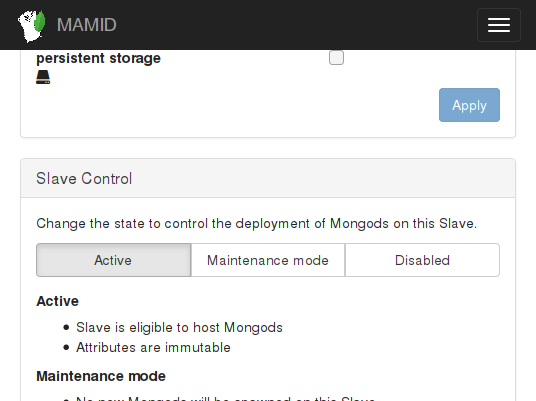
\includegraphics[width=\linewidth, frame]{assets/buttons_closeup}
            \end{column}
        \end{columns}
        
    \end{frame}
    
     \begin{frame}{Controlling Deployment: Screenshots} % this slide gives an impression on how to think when administering MAMID: manipulate constraints, not take direct actions
        \includegraphics<1>[width=\linewidth, frame]{assets/degraded_repl_set}
        \framebreak
        \includegraphics<2>[width=\linewidth, frame]{assets/unreachable_slave}
        \framebreak
        \includegraphics<3>[width=\linewidth, frame]{assets/slave_changing_state}
        \framebreak
        \includegraphics<4>[width=\linewidth, frame]{assets/repl_set_repair1}
        \includegraphics<5>[width=\linewidth, frame]{assets/repl_set_repair2}
        \includegraphics<6>[width=\linewidth, frame]{assets/repl_set_repair3}
        \framebreak
    \end{frame}
    
    \againframe<10-13>{reqanalysis}
    
    \begin{frame}{Monitoring \& Alerting}
        \begin{itemize}
            \item declarative administration $\implies$ infrastructure description
            \item zero-configuration monitoring \pnote{emphasize it is built in}
            \item HTTP API: decouple monitoring \& alerting \pnote{expose recognized problems through an HTTP API}
            \begin{itemize}
                \item MAMID \textit{notifier} supports e-mail notifications
                \item easy integration into existing infrastructure possible \pnote{HTTP API also allows easy integration into existing monitoring frameworks \& alerting services, e.g. Pager Duty, Pushover or similar}
            \end{itemize}
        \end{itemize}
    \end{frame}
    
   \againframe<13-18>{reqanalysis}
    
    \begin{frame}
        \frametitle{Implementation Constraints}
        \begin{itemize}
            \item<2-> Primary target OS: OpenIndiana 105a9
            \item<3-> Frontend \begin{itemize}
            	\item AngularJS
            	\item Bootstrap
            \end{itemize}
            \item<4-> Core Application: Go $>=$ 1.6
            \begin{itemize}
                \item<5-> compiled language, good performance
                \item<6-> built-in concurrency paradigm (channels)
                \item<7-> rich standard library
                \item<8-> cross-platform, simple cross-compilation \pnote{solves problem of missing C++ 11 support in the C++ compiler on the cluster}
                \item<9->\texttt{\$ GOOS=solaris go build}
            \end{itemize}
        \end{itemize}
        
    \end{frame}
        
   
     % end of requirement analysis
    
    \againframe<3>{waterfall}
    \section{Application Design}
    
    \begin{frame}[label=appdesign]{Application Design}
          \includegraphics[width=\linewidth]{assets/class_diagram.pdf}
    \end{frame}
       
   \begin{frame}{Master Slave Protocol}
       \begin{itemize}
           \item HTTP(S) based protocol
           \item JSON transport format
           \item x.509 client certificate authentication\footnote{OpenSSL-based CA scripts already prepared.}
           \item Central idea: communicating state, not commands\footnote{more on this later}
           \begin{itemize}
               \item Process states
               \item Abstract Mongod configuration
            \end{itemize}
        \end{itemize}
    \end{frame}
    
    \againframe{appdesign}

    \begin{frame}{Slave}
        
           \begin{itemize}
               \item Runs on every cluster host
               \item Unprivileged daemon
               \item MSP listener
               \item Mongod process management
               \item Idempotent (re)configuration of Mongods
            \end{itemize}
            \vspace{15pt}
            \texttt{\$ mamid\_slave -listen ':8081' -data /srv/mamid/data}
    \end{frame}
    
    \againframe{appdesign}
    
    \begin{frame}{Master}
        
        \begin{itemize}
            \item Runs on central instance, e.g. gateway host
            \item MSP client
            \item PostgreSQL as backing store for data
            \item Repository pattern: \textit{independent} components communicate through data in DB
            \begin{description}
                 \item[Allocator]: determines cluster layout (deployment of Mongods)
                 \item[Deployer]: sends desired configuration state to slaves\pnote{thus enforces the cluster layout}
                 \item[Monitor]: continuous monitoring (observed state)
                 \item[REST API]: documented interface toward the user
            \end{description}
            \item HTTPS \& TLS client authentication\pnote{again, the OpenSSL-scripts are already prepared. No reason not to set this up.}
        \end{itemize}
        \vspace{15pt}
        \texttt{\$ mamid\_master -listen ':8080' -db.dsn '<Postgres dsn>'}
        
    \end{frame}
    
    \againframe{appdesign}
    
    \begin{frame}{GUI}
           HTML5/CSS3/JS frontend with master's REST API
           \begin{itemize}
	           	\item AngularJS MVC pattern \pause
	           	\item Model implicitly derived from API JSON objects \pause
	           	\item View: HTML + CSS \pause
	           	\item Controller: JavaScript evaluated by the web browser
           \end{itemize}
    \end{frame}
    
    \againframe{appdesign}
    
    \begin{frame}{Notifier}
        
        \begin{itemize}
            \item Polls the master's REST API
            \item Configurable list of alert contacts
            \begin{itemize}
                \item currently limited to e-mail
                \item support for SMTP \textit{smarthost}
            \end{itemize}
            \item Extensible to support other notification mechanisms %TODO correct preposition?
        \end{itemize}
        \vspace{15pt}
        \texttt{\$ mamid\_notifier /etc/mamid/notifier.conf}
    \end{frame}
    
    \againframe{appdesign}
    
    % end of application design phase
    
    \againframe<4>{waterfall}
    
    \section{Implementation \& Testing (Part I)}\pnote{mention two phases were merged for a more flexible schedule}
    
    \begin{frame}{Checkmarks First}
        \begin{itemize}
            \item All mandatory criteria implemented \only<2->{\done}
            \item Some optional criteria implemented \only<3->{\done}
            \item Unforeseen features added \only<4->{\done}
            \item Deadlines met \only<5->{\done}
            \item Sleep deprivation \only<6->{\done}
            \item Caffeine addiction \only<7->{\done}
            \item Software works and is useful \only<8->{\done}
        \end{itemize}
    \end{frame}
    
    \begin{frame}{Development Workflow}
        Tools \& Infrastructure
        \begin{itemize}
            \pause \item Git + GitHub
            \pause \item Self-hosted Continuous Integration (Jenkins, both Linux \& OpenIndiana)
            \pause \item Feature branches \& \texttt{master} branch protection
            \pause \item Unified code style (\texttt{gofmt})
            \pause \item Static code-analysis (\texttt{go vet})
            \pause \item Unit testing (\texttt{go test})
            \pause \item Coverage profiles as CI artifacts (\texttt{go cover})
            \pause \item Local staging environment (Docker)
            \pause \item All of the above wrapped in a GNU Makefile
            \pause \item Dog-fooding the master API for manual tests (Python)
        \end{itemize}
    \end{frame}
   \begin{frame}{Communication}
        \begin{itemize}
            \pause \item GitHub's issue tracker
            \pause \item Slack platform
            \begin{itemize}
                \pause \item Commit \& Repo activity bot
                \pause \item CI results bot
            \end{itemize}
        \end{itemize}
    \end{frame}
    
    \begin{frame}[allowframebreaks]{Distribution of Work}
        
        \begin{columns}
            \begin{column}{0.5\linewidth}
                \centering
                \begin{figure}[h]
                    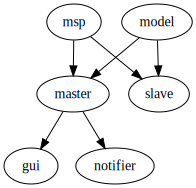
\includegraphics[width=\linewidth]{assets/module_graph.eps}
                    \caption{Module Dependency Graph}
                \end{figure}
            \end{column}
           
            \begin{column}{0.5\linewidth}
                 \centering
                 \begin{figure}[h]
                     \begin{tabular}{l|l}
                         \toprule
                         Component & Name\\
                         \midrule
                         msp       & Anton\\
                         model     & Christian\\
                         master    & Anton, Christian\\
                         slave     & Bob\\
                         gui       & Janis\\
                         notifier  & Niklas, Janis\\
                         \bottomrule
                        \end{tabular}
                        \caption{Distribution of Work}
                    \end{figure}
            \end{column}
        \end{columns}
        
    \end{frame}
    \begin{frame}{Distribution of Work}
        
        Module development
        
        \begin{itemize}
            \pause \item Attempt to distribute work fairly among members
            \pause \item Independent work
            \begin{itemize}
                \item Different schedules
                \item Everyone stays informed
            \end{itemize}
        \end{itemize}
        
        \pause
        Integration
        
        \begin{itemize}
            \item Distributed application
            \item Problems encountered in this phase
            \begin{description}
                \pause \item [model] additional data types
                \pause \item[msp] additional method (Replica Set initiation)
                \pause \item[gui] more linking between detail views, convenience features
                \pause \item[notifier] mail server configuration $\rightarrow$ configuration file
                \pause \item[slave] unexpected MongoDB behavior
                \pause \item[master] ORM layer problems, prioritization data structures
            \end{description}
        \end{itemize}
        
         \pnote{msp and model were easy to implement. initial versions finished after a few days.}
         \pnote{master repository pattern proved more difficult than expected, mostly because of immature ORM layer (would use something more lightweight / direct SQL instead). More on this later}
         \pnote{initial slave implementation was finished early, however, required substantial rewriting after discovering unexpected behavior in the MongoDB configuration process}
         \pnote{notifier \& GUI implementation were straightforward because of well-defined API interface. actual GUI has way more features than GUI drafts in the functional spec }
        
    \end{frame}
    
    \begin{frame}{Statistics}
        \pause
        \begin{figure}[h]
            \centering
            \begin{tabular}{lllll}
                \toprule
                files  &  language  &  blank  &  comment  &  code \\
                \midrule
                71  &  Go  &  2102  &  923  &  9497 \\
9  &  JavaScript  &  121  &  534  &  1049 \\
9  &  HTML  &  24  &  6  &  846 \\
4  &  CSS  &  87  &  49  &  304 \\
4  &  SQL  &  115  &  97  &  284 \\
2  &  Markdown  &  80  &  0  &  188 \\
3  &  Bourne Shell  &  8  &  1  &  48 \\
2  &  make  &  11  &  0  &  28 \\
1  &  Python  &  5  &  2  &  21 \\
1  &  Bourne Again Shell  &  4  &  3  &  3 \\

                \bottomrule
            \end{tabular}
            \caption{Lines of Code in the code repository. \\ Generated by \textit{generate\_report.bash} with \texttt{cloc(8)}. Commit \texttt{6465447}}
        \end{figure}
    \end{frame}
    \begin{frame}{Statistics}
        \pause
        
        \begin{itemize}
            \item Number of commits: 811
            \item Number of issues: 58 (13 open / 45 closed) \pnote{mention number of open issues mostly enhancements, 13 not a bad sign }
        \end{itemize}
        
        \pause

        \begin{figure}
        \centering
        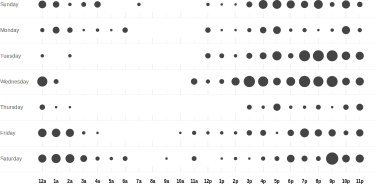
\includegraphics[width=0.6\linewidth]{assets/gh_punchcard}
        \caption{GitHub Punchcard \texttt{code} repo, commit \texttt{6465447}}
        \label{fig:ghpunchcard}
        \end{figure}
        
        \begin{tiny}
        All data extracted from GitHub, 10 Sep 2016 01:00 CEST 
        \end{tiny}
    
    \end{frame}
    \begin{frame}{Statistics}
        \pause
        \begin{figure}[h]
            \centering
            \begin{tabular}{l|l}
            \toprule
            Module  &  Number of Tests \\
            \midrule
            master & 57 \\
            model & 11 \\
            msp & 0 \\
            notifier & 16 \\
            slave & 5 \\
            \bottomrule
            \end{tabular}
            \caption{Number of tests by module.\\Generated by \textit{generate\_report.bash}. Commit \texttt{6465447}}
        \end{figure}
        
    \end{frame}
    \begin{frame}[fragile]{Statistics}

\texttt{go cover} (formatted)
\begin{verbatim}
ok  	master            6.361s	coverage: 45.3% of statements
?   	master/cmd        [no test files]
ok  	master/masterapi  36.568s	coverage: 56.1% of statements
ok  	model             8.559s	coverage: 29.6% of statements
?   	msp	              [no test files]
ok  	notifier          0.006s	coverage: 40.0% of statements
ok  	slave             0.086s	coverage: 19.5% of statements
\end{verbatim}

\begin{itemize}
    \item Tests against ORM layer
    \item Time constraints
    \item Complex fixtures for \texttt{ClusterAllocator}, \texttt{Deployer}, \texttt{Monitor}
    \item $\rightarrow$ only prepare testing infrastructure
\end{itemize}

\end{frame}
    
    \section{Live Demo}    
    
        \againframe<4>{waterfall}
    \section{Implementation \& Testing (Part II)}
   
    \begin{frame}{Lessons Learned}
     
      ORM layers \& Go
            
      \pnote{as already suggested before the demo, implementing master \& slave proved difficult}
      \pause
      \begin{itemize}
        \item<+-> Generally debatable\footnote{\tiny Recommended read: \url{http://www.hydrogen18.com/blog/golang-orms-and-why-im-still-not-using-one.html}}
        \item<+-> Lack of dynamism in language $\rightarrow$ transparent lazy fetching impossible
        \item<+-> \texttt{database/sql} transaction support \pnote{cannot set isolation level through standard db.Begin() interface}
        \item<+-> \texttt{gorm} shortcomings
          \begin{itemize}
            \item<+-> missing foreign key support $\rightarrow$ ugly hacks \pnote{mention no ON DELETE CASCADE} 
            \item<+-> missing fine-grained \texttt{UPDATE}s with complex object graphs
          \end{itemize}
      \end{itemize}

    \end{frame}
    \begin{frame}{Lessons Learned}

      MongoDB \pause \shrug \pause

      \begin{itemize}
       \item<+-> Good documentation
       \item<+-> Focus on manual configuration \pnote{no automation} \pnote{no automation} \pnote{no automation} \pnote{no automation}
       \item<+-> No OpenSSL support in Solaris builds
       \item<+-> $\rightarrow$ no x.509 support on Solaris
       \item<+-> $\rightarrow$ keyfile authentication in production
       \item<+-> Replica Set Configuration
         \begin{itemize}
           \item<+-> Initiation from single Mongod
           \item<+-> $\rightarrow$ global coordination in master
                   \pnote{does not fit with original architecture, had to extend MSP \& deployer for this special case, leaky abstractions}
         \end{itemize}
      \end{itemize}

    \end{frame}
    \begin{frame}{Lessons Learned}
      \begin{figure}
        \centering
        \includegraphics[height=0.6\textheight]{assets/mongod_states_old}
              \caption{Mongod Configuration States (pre-implementation)}
        \label{fig:mongodstates}
        \end{figure}
    \end{frame}
    \begin{frame}{Lessons Learned}
      \begin{figure}
        \centering
        \includegraphics[height=0.8\textheight]{assets/mongod_states}
              \caption{Mongod Configuration States (post-implementation)}
        \label{fig:mongodstates}
        \end{figure}
    \end{frame}
\begin{frame}{Lessons Learned}

      Operational Needs - Exposing more Information

      \pnote{intention: give admin insight into the deployment}  
      \pause
      \begin{itemize}
              \item<+-> Mongods by slave \& Replica Set
              \item<+-> Hyperlinks between slave \& Replica Set
              \item<+-> Visualize problems in slave \& Replica Set view
              \item<+-> Copy-to-clipboard command lines \& Mongo shell commands
      \end{itemize}
     
    \end{frame}

    \begin{frame}{What Worked Well}
            \begin{columns}
            \begin{column}{0.6\linewidth}
              \begin{itemize}
                \item<2-> Go
                    \begin{itemize}
                      \item<3-> \texttt{net/http}
                      \item<4-> \texttt{crypto/tls}
                      \item<5-> channels + \texttt{sync}
                      \item<6-> \texttt{flags}
                      \item<7-> code organization
                      \item<8-> \texttt{go(8)} (build system, testing, vet)
                    \end{itemize}
                \item<9-> PostgreSQL $>>$ SQlite \pnote{originally SQLite, but locking behavior not suitable with repository pattern + concurrent access}
                \item<10-> AngularJS \pnote{Angular maaaaagic (nicely integrated mvc) saves a lot of time}
                \item<11-> Bootstrap \pnote{familiar, nice looking user interfaces. UI components. accessibility + readability}
                \item<12-> Docker \pnote{Docker, in particular for testing networked applications}
                \item<13-> Jenkins (testing on OpenIndiana)
                \item<14-> Slack (convenience)
                \item<15-> \LaTeX + \texttt{git} <3
              \end{itemize}
            \end{column}
            \begin{column}{0.4\linewidth}
                \begin{tabular}{ll}
                        \visible<9->{
\includegraphics[width=0.35\linewidth]{assets/contrib/postgres/PostgreSQL_logo}} & \visible<2->{
\includegraphics[width=0.4\linewidth]{assets/contrib/gopher/gopher}} \\
                        \visible<10->{
\includegraphics[width=0.35\linewidth]{assets/contrib/angularjs/AngularJS_logo}} & \visible<12->{
\includegraphics[width=0.35\linewidth]{assets/contrib/docker/vector_h-trans.eps}} \\
                \end{tabular}
            \end{column}
        \end{columns}

    \end{frame}
    
    \againframe<5>{waterfall}
    
    \section{Review on PSE}

    \newcommand\itembad{\item[\notdone]}
    \newcommand\itemgood{\item[\done]}

    \begin{frame}{Review on PSE}
      \pause
      \begin{itemize}
        \itembad<+-> Waterfall development model
        \begin{itemize}
          \itembad<+-> Immutable document artifacts
          \itembad<+-> Split between \textit{implementation} \& \textit{testing}
          \itembad<+-> $\rightarrow$ cross-component bugs discovered too late
        \end{itemize}
        \itembad<+-> UML
            \begin{itemize}
              \item class diagrams
              \item activity diagrams: helpful
            \end{itemize}
        \itembad<+-> Time vs ECTS
        \itembad<+-> Final PSE phases overlap with examination phase
        \itemgood<+-> Project in English
        \itemgood<+-> Software might actually be used!
      \end{itemize}
    \end{frame}

    \begin{frame}{}
       \vfill
        \centering
        \Huge
        Q\&A \\
            \vspace{10pt}
            \hspace*{5pt}
\includegraphics[width=0.3\linewidth]{assets/mamid3_web}
        \vfill
    \end{frame}
    
\end{document}


